\section{Overview of Results. Demonstration of Project}
% 
Show gif/PPM sequence to demonstrate flocking 

% 
Talk about variable parameters \\
\texttt{
num\_boids \\
perception\_radius \\
num\_threads \\
}

% Per-frame latency 
Figure~\ref{fig:framelatency} shows the latency incurred in performing computations and rendering each frame for a simulation of 1000 frames with varying number of boids. For a given simulation, the plot shows that per-frame latency is fairly consistent over time, and flocking performance can therefore be evaluated using average metrics such as frame rate (FPS). The plot also shows that naïve CPU-based boid-flocking scales poorly with increasing number of boids.

\begin{figure}[ht!]
\centering
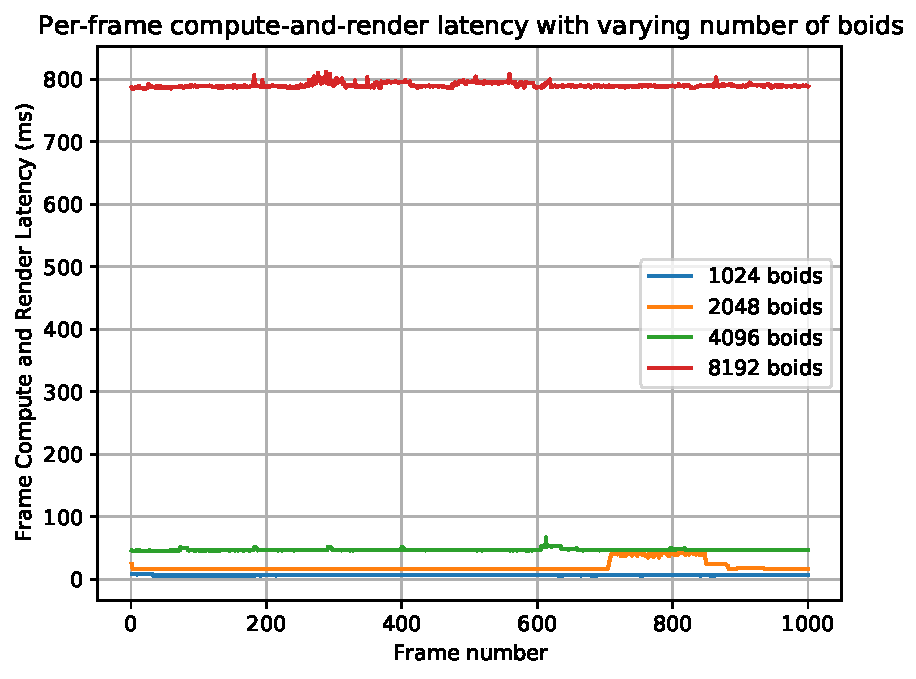
\includegraphics[scale=0.8]{plots/latency-per-frame.pdf}
\caption{Time taken to compute and render each frame in milliseconds for a naïve CPU-based implementation.}
\label{fig:framelatency}
\end{figure}
